\section{Interprozesskommunikation}

\subsection{Semaphore}

Semaphor ist ein Signalisierungsmechanismus (signaling mechanism), bestehend aus einer P-Operation (proberen, prüfen, reservieren) und V-Opration (verhogen, erhöhen, freigeben).

Binäre Semaphore:

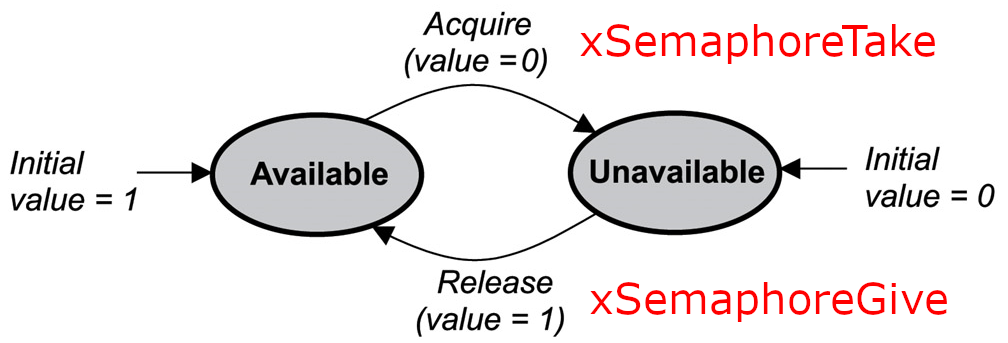
\includegraphics[width=\linewidth]{Binary_Semaphore.png}

Counting Semaphore:

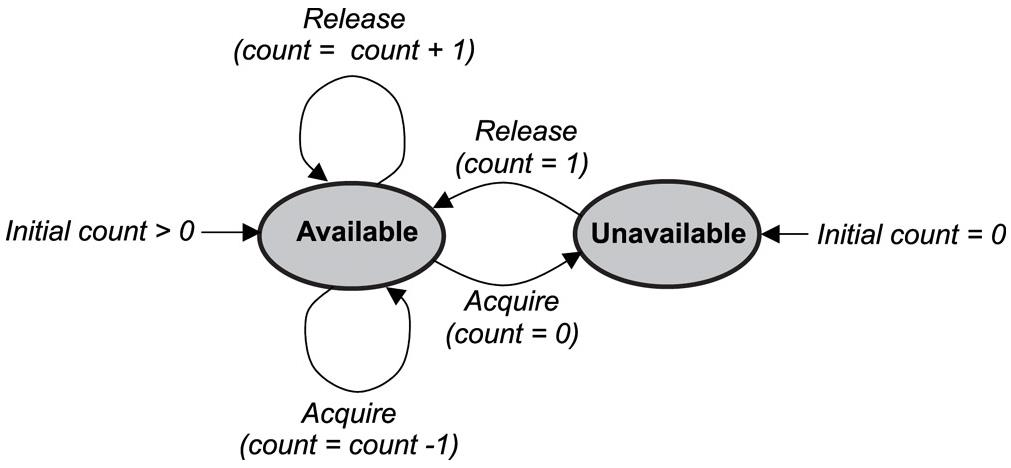
\includegraphics[width=\linewidth]{Counting_Semaphore.png}

\subsection{Mutual Exclusion (Mutex) Semaphore}

Mutex ist ein Sperrmechanismus (locking mechanism), welcher den Wert 0 und 1 annehmen kann.
Key words: Ownership, Recursive Locking, Task Deletion Safety, Priority Inversion Avoidance.
Recursive mutexes can be locked and unlocked multiple times by the task that owns them.

Siehe auch Abschnitt \ref{sec:semaphore_api}.


\subsection{Synchronisation}

\begin{center}
    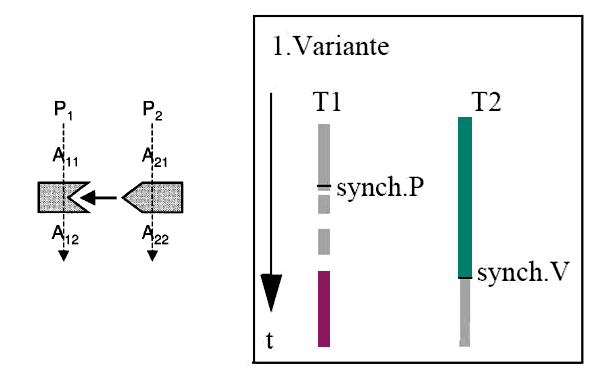
\includegraphics[width=.8\linewidth]{semaphore_sync1.png}

    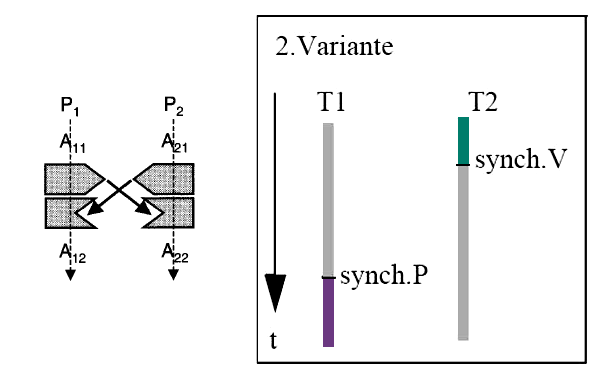
\includegraphics[width=.8\linewidth]{semaphore_sync2.png}
\end{center}


